% !TeX root = ../artigo.tex
\section{SERVIDOR OPENLDAP}

Nesta seção, será descrito detalhadamente o processo de instalação dos pacotes e componentes necessários para configurar o ambiente virtual Debian, de forma que funcione como um servidor LDAP, que será usado para manter as informações nele inseridas. 

Além disso serão demonstradas, as configurações necessárias para que o LAM (LDAP Account Manager), uma ferramenta de gerenciamento de contas LDAP, seja capaz de administrar as informações no diretório.

\subsection{INSTALAÇÃO DOS PACOTES E COMPONENTES}

Os pacotes e componentes que serão instalados são essenciais para o funcionamento do ambiente. A seguir, serão explicados cada um desses pacotes em detalhes, e seu papel na infraestrutura do projeto.

O primeiro passo é a instalação dos componentes, como descrito no código abaixo, que em conjunto formam a base para criar um ambiente web, que servirá de base para hospedar o LAM.

\begin{lstlisting}
    sudo apt install apache2 php php-cgi libapache2-mod-php php-mbstring php-common php-pear -y
\end{lstlisting}

Cada pacote instalado a partir desse comando, podem ser descritos abaixo como:

\begin{itemize}
    \item apache2: O Apache é um servidor web que lida com solicitações de páginas da web e as envia aos navegadores dos clientes.
    \item php: PHP é uma linguagem de programação do lado do servidor que permite criar páginas web dinâmicas e interativas.
    \item php-cgi: O PHP-CGI é um interpretador que permite ao servidor web (como o Apache) processar scripts PHP.
    \item libapache2-mod-php: Este módulo do Apache integra o PHP ao servidor, permitindo a execução de scripts PHP.
    \item php-mbstring: A extensão mbstring ajuda a lidar com caracteres e texto multibyte em diferentes idiomas.
    \item php-common: O pacote php-common contém recursos e configurações compartilhadas necessárias para o PHP funcionar corretamente.
    \item php-pear: O PEAR é um sistema de gerenciamento de pacotes que fornece bibliotecas e extensões adicionais para expandir a funcionalidade do PHP.
\end{itemize}

Esses componentes trabalham em conjunto para criar um ambiente web flexível e poderoso. O Apache gerencia as solicitações e respostas HTTP, enquanto o PHP processa scripts e gera conteúdo dinâmico. As extensões e módulos adicionais, adicionam funcionalidades extras para atender a diversas necessidades de desenvolvimento web.

Finalizado o processo de instalação do ambiente web, foi realizada  a instalação dos pacotes essenciais relacionados ao LDAP.

\begin{lstlisting}
    sudo apt install slapd ldap-utils -y
\end{lstlisting}

Este comando desempenha um papel crucial na configuração do ambiente, instalando o servidor LDAP ("slapd") e um conjunto de ferramentas úteis para interagir com ele ("ldap-utils"). Como visto na figura \ref{fig:compLDAP} o SLAPD, é o principal Daemon responsável pelas funções do servidor.

A partir do comando abaixo é possível extrair dados de um servidor LDAP e exibé-los no formato LDIF (LDAP Data Interchange Format) no terminal. O LDIF é um formato de texto que representa as entradas e informações armazenadas em um diretório LDAP.

\begin{lstlisting}
    sudo slapcat
\end{lstlisting}

\begin{figure}[h]
	\centering
	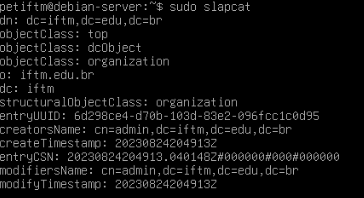
\includegraphics[scale=0.8]{textuais/codigo3.png}
	\caption{Retorno do comando "sudo slapcat"
	\label{fig:sudoslapcat}}
\end{figure}

Após realizada a instalação do servidor LDAP, foi realizada através do comando abaixo, a instalação do pacote do LAM no sistema, que como mencionado anteriormente, é uma ferramenta útil para administrar e simplificar o gerenciamento de contas por meio de uma interface web.

\begin{lstlisting}
    sudo apt install ldap-account-manager -y
\end{lstlisting}

Conforme instalado o pacote, o próximo passo foi a configuração do servidor Apache para trabalhar de forma adequada com o PHP-CGI, garantindo que os scripts PHP sejam processados corretamente. Eles garantem que o servidor seja capaz de suportar corretamente o módulo do LAM.

\begin{lstlisting}
    sudo a2enconf php*-cgi
    sudo systemctl reload apache2
    sudo systemctl enable apache2
\end{lstlisting}

Os comandos acima também recarregam e garantem que o Apache seja inicializado automaticamente, sempre que o sistema for reiniciado, proporcionando alta disponibilidade à interface web do LAM. Além disso, a partir do comando abaixo, é possível verificar o status do serviço do servidor web Apache no sistema.

\begin{lstlisting}
    sudo systemctl status apache2
\end{lstlisting}

\begin{figure}[h]
	\centering
	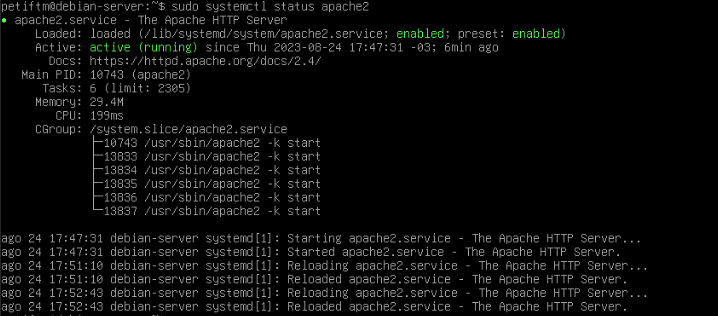
\includegraphics[scale=0.7]{textuais/codigo5.png}
	\caption{Retorno do comando "sudo systemctl status apache2"
	\label{fig:status}}
\end{figure}

Como configuração adicional, também foi atribuído à maquina virtual Debian um endereço IP estático, para que sempre seja possível acessar a interface web, pelo mesmo endereço em outras máquinas da mesma rede. Essa configuração pode ser feita a partir do comando para a modificação do arquivo abaixo.

\begin{lstlisting}
    nano /etc/network/interfaces
\end{lstlisting}

\begin{figure}[h]
	\centering
	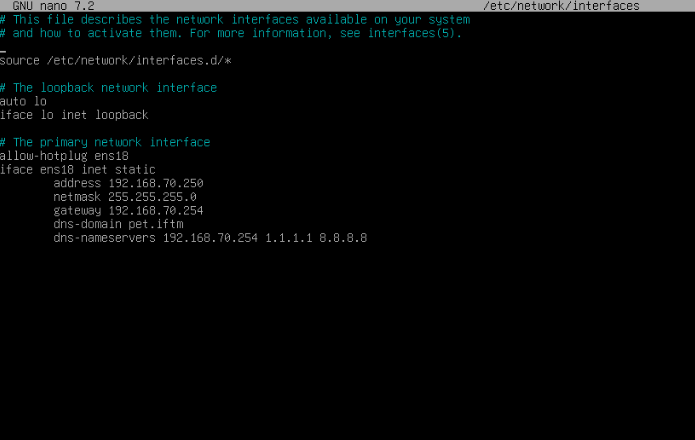
\includegraphics[scale=0.6]{textuais/codigo7.png}
	\caption{Arquivo "/etc/network/interfaces"
	\label{fig:network}}
\end{figure}

\subsection{CONFIGURAÇÃO DO LDAP ACCOUNT MANAGER}

Ao acessar a interface web do LAM, ilustrada na figura \ref{fig:LAM1} abaixo, pelo endereço do servidor definido ("http://IP-Server/lam), foram necessárias configuração dos perfis de servidor para o funcionamento do gerenciador, a partir da aba "LAM configuration".

\begin{figure}[h]
	\centering
	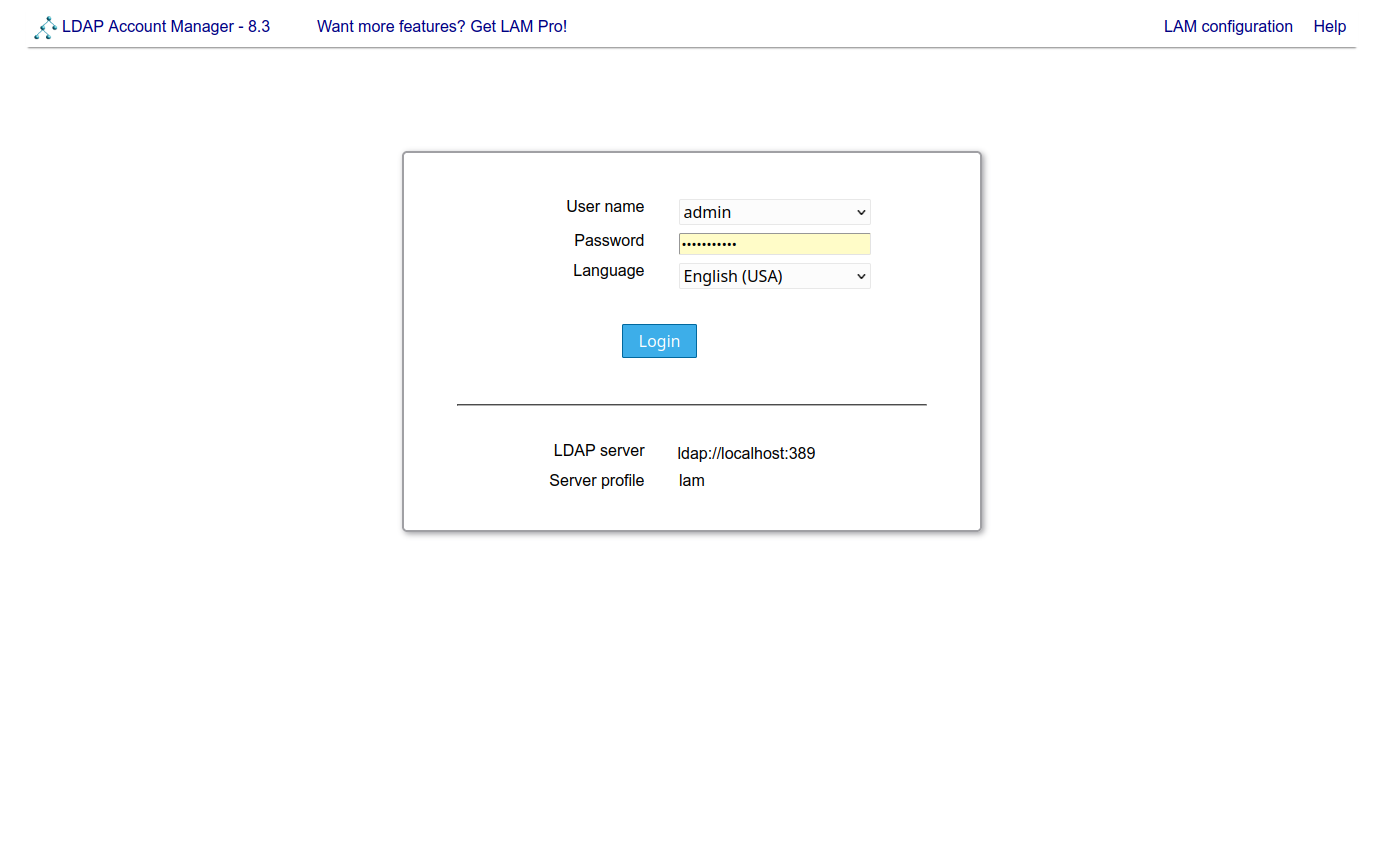
\includegraphics[scale=0.3]{textuais/LAMNovo.png}
	\caption{Tela inicial do LDAP Account Manager
	\label{fig:LAM1}}
\end{figure}

As configurações realizadas na aba de "General Settings", incluem a alteração do "Tree Sufix" para o sufixo do domínio anteriormente estabelecido, a "List of Valid Users" para o sufixo da conta de admin criada, além da definição de uma nova senha para a conta padrão LAM utilizada. 

Além dessas configurações, também foram alterados os sufixos dos tipos de conta existentes no servidor, para os sufixos correspondentes às configurações feitas. Alterações essas demonstradas abaixo nas figuras \ref{fig:LAM4} e \ref{fig:LAM5}.

\begin{figure}[ht]
    \begin{subfigure}{0.48\textwidth}
    	\centering
    	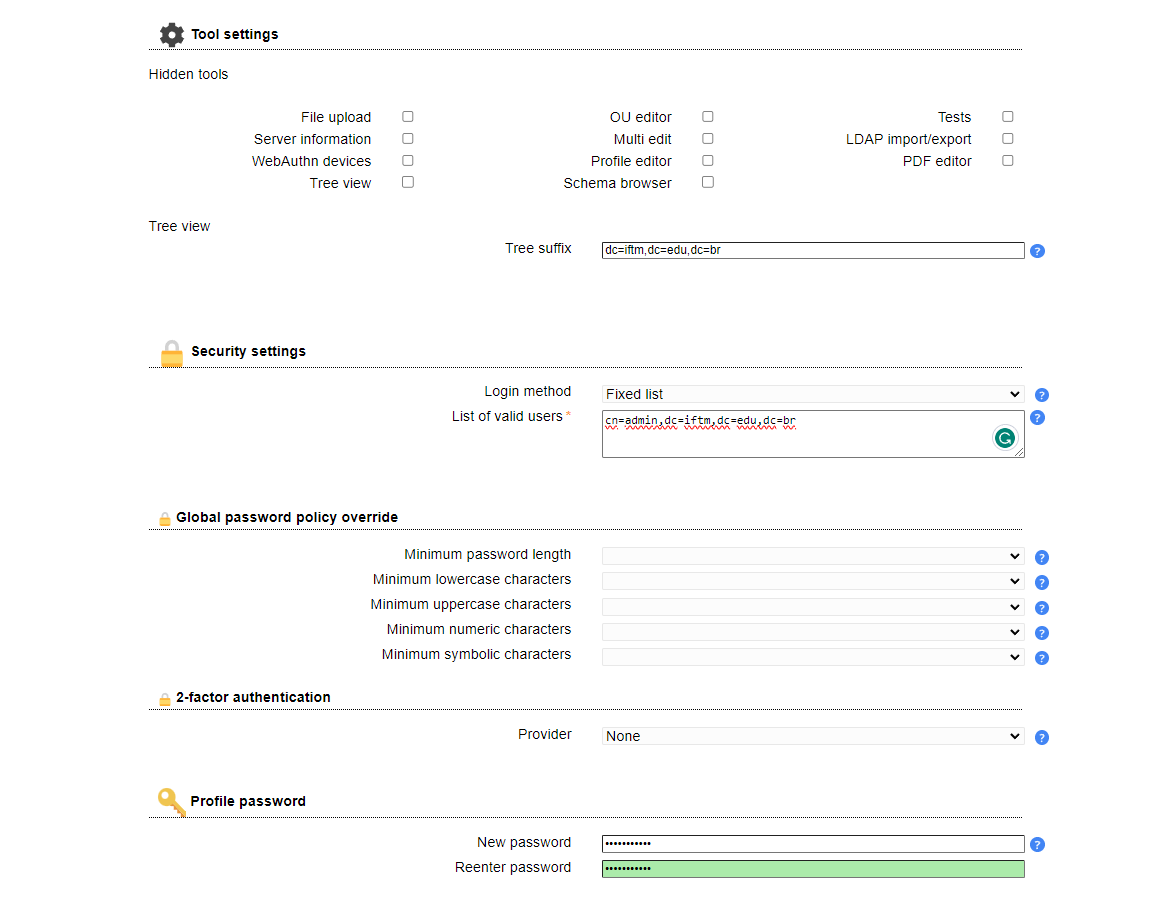
\includegraphics[width=\linewidth]{textuais/LAM4.png}
    	\caption{Configurações gerais do LAM
    	\label{fig:LAM4}}
    \end{subfigure}%
    \hspace{0.04\textwidth} % Espaço horizontal
    \begin{subfigure}{0.48\textwidth}
    	\centering
    	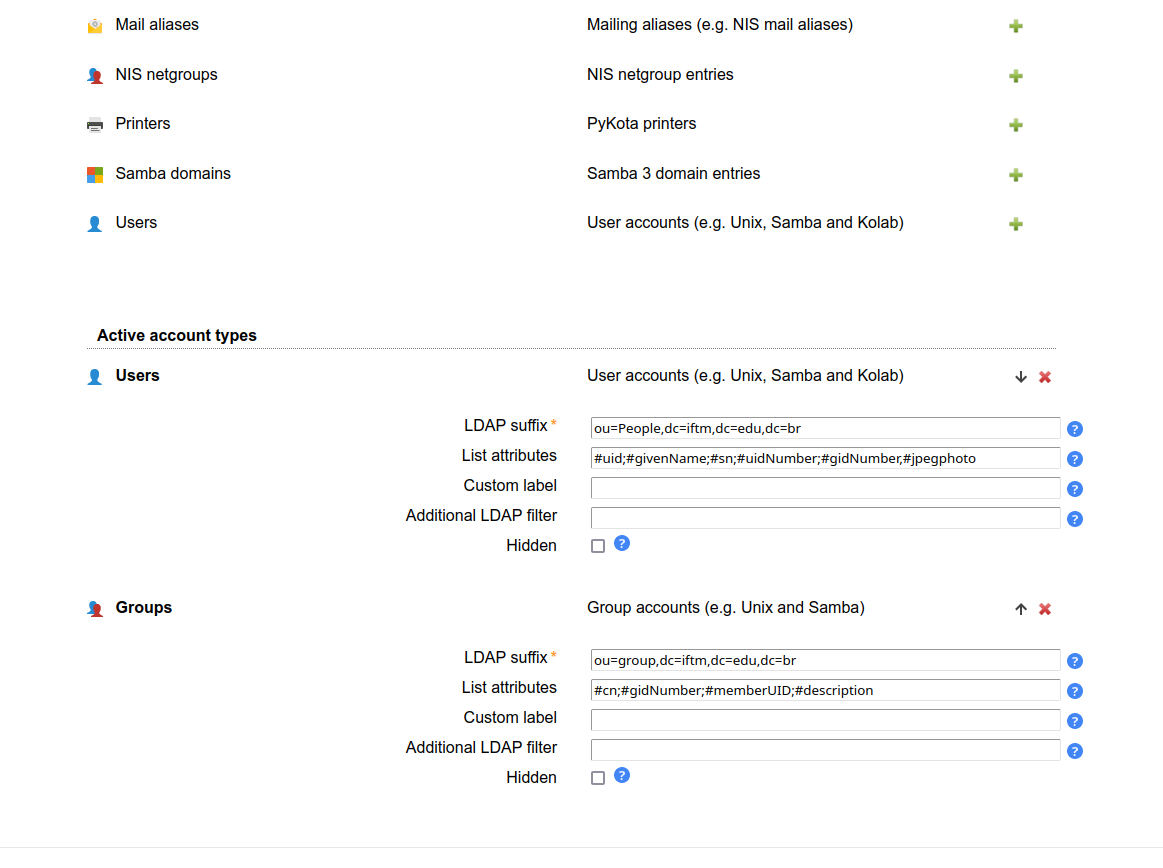
\includegraphics[width=\linewidth]{textuais/TiposContaLAM.png}
    	\caption{Configurações de tipos de conta do LAM
    	\label{fig:LAM5}}
    \end{subfigure}
    \caption{Configuração dos perfis de servidor}
    \label{fig:figurasLAM}
\end{figure}

Realizadas as configurações adequadas, o servidor ficou pronto para receber as informações de contas de usuários, ou grupos como ilustrado na figura \ref{fig:LAM6}. Após isso, foram criados os perfis de cada usuário a fim de validar seu devido funcionamento.

\begin{figure}[h]
	\centering
	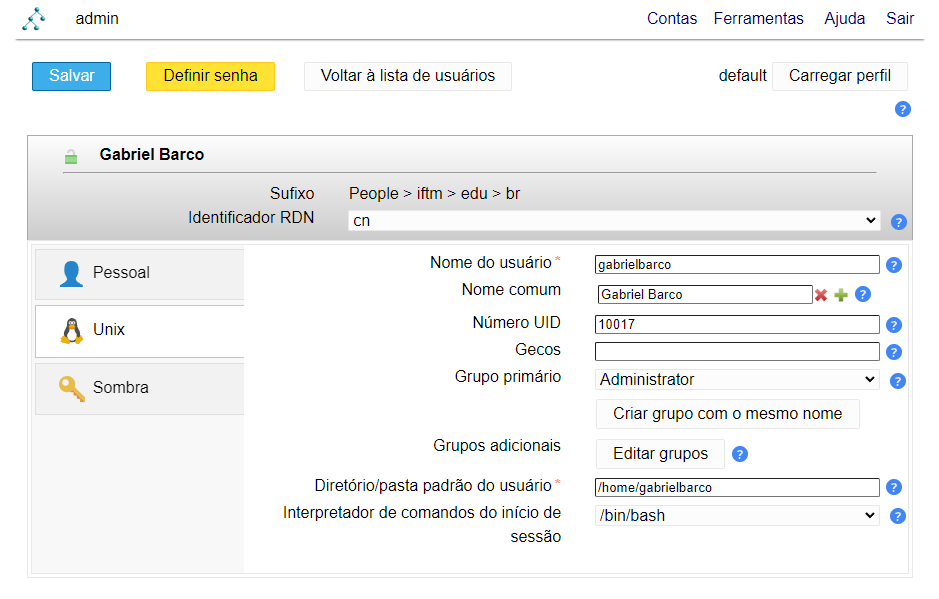
\includegraphics[scale=0.4]{textuais/CriaçãoUsuario.png}
	\caption{Tela de criação de usuário
	\label{fig:LAM6}}
\end{figure}

Com a criação completa, os perfis também podem ser vizualizados tanto na interface do LAM, quanto pela extração direta dos dados do servidor LDAP, com o uso do comando "slapcat", como demonstrado na figura \ref{fig:sudoslapcat}.